\documentclass[a4paper, titlepage, oneside, 12pt]{article}%      autres choix : book  report

\usepackage[utf8]{inputenc}%           gestion des accents (source)
\usepackage[T1]{fontenc}%              gestion des accents (PDF)
\usepackage[francais]{babel}%          gestion du français
\usepackage{textcomp}%                 caractères additionnels
\usepackage{mathtools,  amssymb, amsthm}% packages de l'AMS + mathtools
\usepackage{lmodern}%                  police de caractère
\usepackage{geometry}%                 gestion des marges
\usepackage{graphicx}%                 gestion des images
\usepackage{xcolor}%                   gestion des couleurs
\usepackage{array}%                    gestion améliorée des tableaux
\usepackage{calc}%                     syntaxe naturelle pour les calculs
\usepackage{titlesec}%                 pour les sections
\usepackage{titletoc}%                 pour la table des matières
\usepackage{fancyhdr}%                 pour les en-têtes
\usepackage{titling}%                  pour le titre
\usepackage[framemethod=TikZ]{mdframed}% print frames
\usepackage{caption}%                  for captionof
\usepackage{listings}%				  pour insertion de codes 
\usepackage{enumitem}%                 pour les listes numérotées
\usepackage{microtype}%                améliorations typographiques
\usepackage{csvsimple}%                convertir un fichier .csv en tableau
\usepackage{url}%					  amélioration afficahge url
\usepackage{hyperref}%                 gestion des hyperliens
\usepackage{svg}	%					  gestion des svg	
\usepackage{float}%					  gestion des figure non flotante

\usepackage{titling} %  				  gestion des subtitles 
\newcommand{\subtitle}[1]{%			  definition d'une nouvelle commande sous-titre
  \posttitle{%
    \par\end{center}
    \begin{center}\large#1\end{center}
    \vskip0.5em}%
}                
\lstset{language=c++}
\definecolor{codegreen}{rgb}{0,0.6,0}
\definecolor{codegray}{rgb}{0.5,0.5,0.5}
\definecolor{codepurple}{rgb}{0.58,0,0.82}
\definecolor{backcolour}{rgb}{0.95,0.95,0.92}
 
\lstdefinestyle{mystyle}{
    backgroundcolor=\color{backcolour},   
    commentstyle=\color{codegreen},
    keywordstyle=\color{magenta},
    numberstyle=\tiny\color{codegray},
    stringstyle=\color{codepurple},
    basicstyle=\footnotesize,
    breakatwhitespace=false,         
    breaklines=true,                 
    captionpos=b,                    
    keepspaces=true,                 
    numbers=left,                    
    numbersep=5pt,
    otherkeywords={uint16_t},                  
    showspaces=false,                
    showstringspaces=false,
    inputencoding=latin1,
    showtabs=false,                  
    tabsize=2
}
\lstset{style=mystyle}

\hypersetup{%
    pdfborder = {0 0 0}
}


                                    
\title{Rapport du Projet PSAR :\\ Dispositif Autonome de Synthèse Sonore}
\subtitle{Encadrant : Hugues Genevois \\ Cahier de Charges}

\author{Pierre Mahé}
\date{\today}

\begin{document}  
 \begin{figure}[b]
	
\includegraphics[width=120px] {upmc_logo.jpg}
	\hspace{7cm}
	\vspace{-2cm}
	
\includegraphics[width=120px] {LogoLAM.jpg}
\end{figure}

\maketitle 
\tableofcontents

\newpage
\section{Introduction}
\subsection{Contexte Global}
\paragraph{}
\textbf{Maîtrise d’œuvre :} Hugues GENEVOIS
\vspace{-5mm}
\paragraph{}
\textbf{Maîtrise d’ouvrage :} Pierre MAHÉ

\paragraph{}
Le projet DASS, Dispositif Autonome de Synthèse Sonore, est une collaboration de Michel RISSE, compositeur de "Décor Sonore" ayant à son actif de nombreuses créations et dispositif sonores, et de Hugues GENEVOIS, chercheur au LAM de L'Institut Jean le Rond d'Alembert.

\paragraph{}
Le projet consiste à mettre en place un dispositif générant du son en prennent en compte sont environnement dans le but de souligner les sons pres-exsitant dans cet environement. Le dispositif recueille les informations a l'aide de capteurs diverses permettant de récupérer les buits ambiant, la luminosité, la tempature.

Dans un premiere tant devrait être la base pour une installation artistique, se deroulant en juillet prochain, dans le cadre d'un festival de musique à Noirlac. Dans un second temps Hugues GENEVOIS et Michel RISSE voudraient réaliser une installation plus importante avec de nombreux dispositifs avec pour chacun d'eux des comportements et des caractéristique propre, pour voir l'interation qu'ils pourraient avoir ensemble et les comportements qui en emergerait.

\subsection{Presentation de la demande}
\paragraph{}
Dans le cadre de mon projet PSAR, mon but etais de créer un premier prototype du projet pour s'en service comme base par la suite.\\
J'avais donc pour mission de créer un dispositif portable interagissant avec son environnement. Ce dispositif doit capter l'environnement a l'aide
Le but du projet est de créer un dispositif portable interagissant avec son environnement. Ce dispositif doit capter l'environnement a l'aide de capteurs : micro, luminosité, température, et humidité. Il devra traiter ces données pour en extraire des informations pertinent sur les changements se produisant autour de lui (chants d'oiseaux, passage d'une personne au alentour...). Grâce à ces informations, il devra synthétiser du son.
\paragraph{}
La synthèse devra être paramétrable, pour permettre au compositeur de modifier
l’influence des différant capteurs sur la synthèse sonore.\\
De plus une interface utilisateur devra être présente permettant au compositeur de simuler des données
captés. Cela lui permettra de faire des expérimentations de sa composition.
\paragraph{}
Dans l’optique de la reproduction de ce dispositif pour des installations plus important. Une procédure devra permettre à un utilisateur de pouvoir reproduire l’ensemble du système, aussi bien niveau matériel que logiciel.
\paragraph{}
Le dispositif devant être portable, le programme doit fonctionner sur une nano-
ordinateur de type \texttt{Udoo Quad}. De plus le langage du programme principal doit etre le 
PureData, pour assurer une maintenabilité et une extensionnalité plus facile.
\subsection{La Carte Udoo}
\paragraph{}
% photo udoo
La carte Udoo est un nano ordinateur embarquant un processeur ARM et la connectique d'un ordinateur classique. Avec une entre et sortie micro. La qualité étant suffisante pour notre projet.\\
La caractéristique de cette carte est d'etre compatible arduino et d'offrir les mêmes connectique qu'une Arduino Mega ce qui permet de simplifier la réception des capteurs ainsi que le d'utiliser les bibliothèques déjà implémenter par la vaste communauté Arduino.\\
La carte utilise une carte micro sd pour stocker ses données, ce qui est également un avantage pour le projet car cela permet de dupliquer la partie software du dispositif avec une simple copie de carte mémoire.\\
Le systeme d'exploitation installer est un version simplifié d'Ubuntu, permettant d'utiliser l’environnement linux.

\subsection{Pure Data}
\subsubsection{Presentation generale}
% logo pure data ou image
\paragraph{}
Pure Data est un logiciel, open source, de programmation graphique pour la creation muscale et multimedia en temps reel. Il permet également de gérer des signaux entrants dans l'ordinateur (signaux de capteurs ou événements réseau par exemple) et de gérer des signaux sortants (par des protocoles de réseau ou protocoles électroniques pour le pilotage de matériels divers).\\
Pure Data est un systeme module où il est possible de definir des sous-modules qu'il est possible de re-utiliser a sa gise dans d'autre programme appelé \texttt{patch}.
En Pure Data tous les objets (modules ou donnée) sont des \texttt{boites}.
Ce langage est un langage tres faiblement typé. Il existe quatres types de données de base:\\
\begin{itemize}
\item \textbf{Les Nombres}, qui peuvent reprensenter des nombres entiers comme à virgules
\item \textbf{Les Message}, qui sont des messages purement textuels 
\item \textbf{Les Symboles}, qui corresponde aux messages mixtes, caractère, chiffre...
\item \textbf{Les Tableaux}, qui sont uniquement des tableaux de nombres.
\end{itemize}
Il exite d'autre type de donnée comme les listes qui même avec une representation interne différante ou message ou symboles sont graphiquement identique a un message (avec comme premier mot \texttt{list}). De plus pour changer une liste en message, il suffit de supprimer ce mot clé.

\paragraph{}
Le Pure Data étant un logiciel orienter interation, il est possible a tous moment de modifier son patch en ajoutant des boites au cours de l'execution du programme, il n'est pas nessesaire de relancer le programme. Cela peut permet de modifier le patch en direct sans avoir l’interruption dans le flux audio sortant.

\paragraph{}
Pure Data a aussi l'avant d'etre facilement documentable car il est possible d'associer à une boite quelconque, une boite d'aide avec une explication et des exemples.\\
Cela s'avaire tres utilie pour la compréhension de certaines boites complexe et permet de bien dissocier code et documentation.
\paragraph{}
Un autre atout de Pd est le nombre de d'outils deja implementé dans le logiciel et les boites creer par la comunoté. Certaine proceder a des traitements complexe, comme la detection en temps reel de frequence ou le filtrage performent.

\subsubsection{Externals}
\paragraph{}
En Pure Data, le stockage de donnee est asses complexe c'est pour cela que pour procéder a des algorithme complexe, il est possible d'avoir recours à des\texttt{Externals}.\\
Les externals sont des boites programmées en \texttt{c++}. 

\paragraph{}
Il existe plusieurs API, dans ce projet nous avons choisi d'utiliser \texttt{Flext} pour ca simplicité d'utilisation. De plus cette API est développé par Thomas GRILL, un des principal contributeur de Pure Data ce qui garantie un plus grande parfaite compatibilité avec Pd et une certaine assurance que l'outils reste longtemps maintenu. La communauté des développeurs Pure Data etant limité (une dizaine de personne a travers le monde), cela a une importance car malheuresement beaucoup d'outils ne son pas maintenu suffisant ou sont souvent obsolète.  


\subsection{Structure du projet}
\paragraph{}
Nous avons décider de diviser le programme en cinq modules pour le cote synthèse.

\begin{figure}
  \centering
  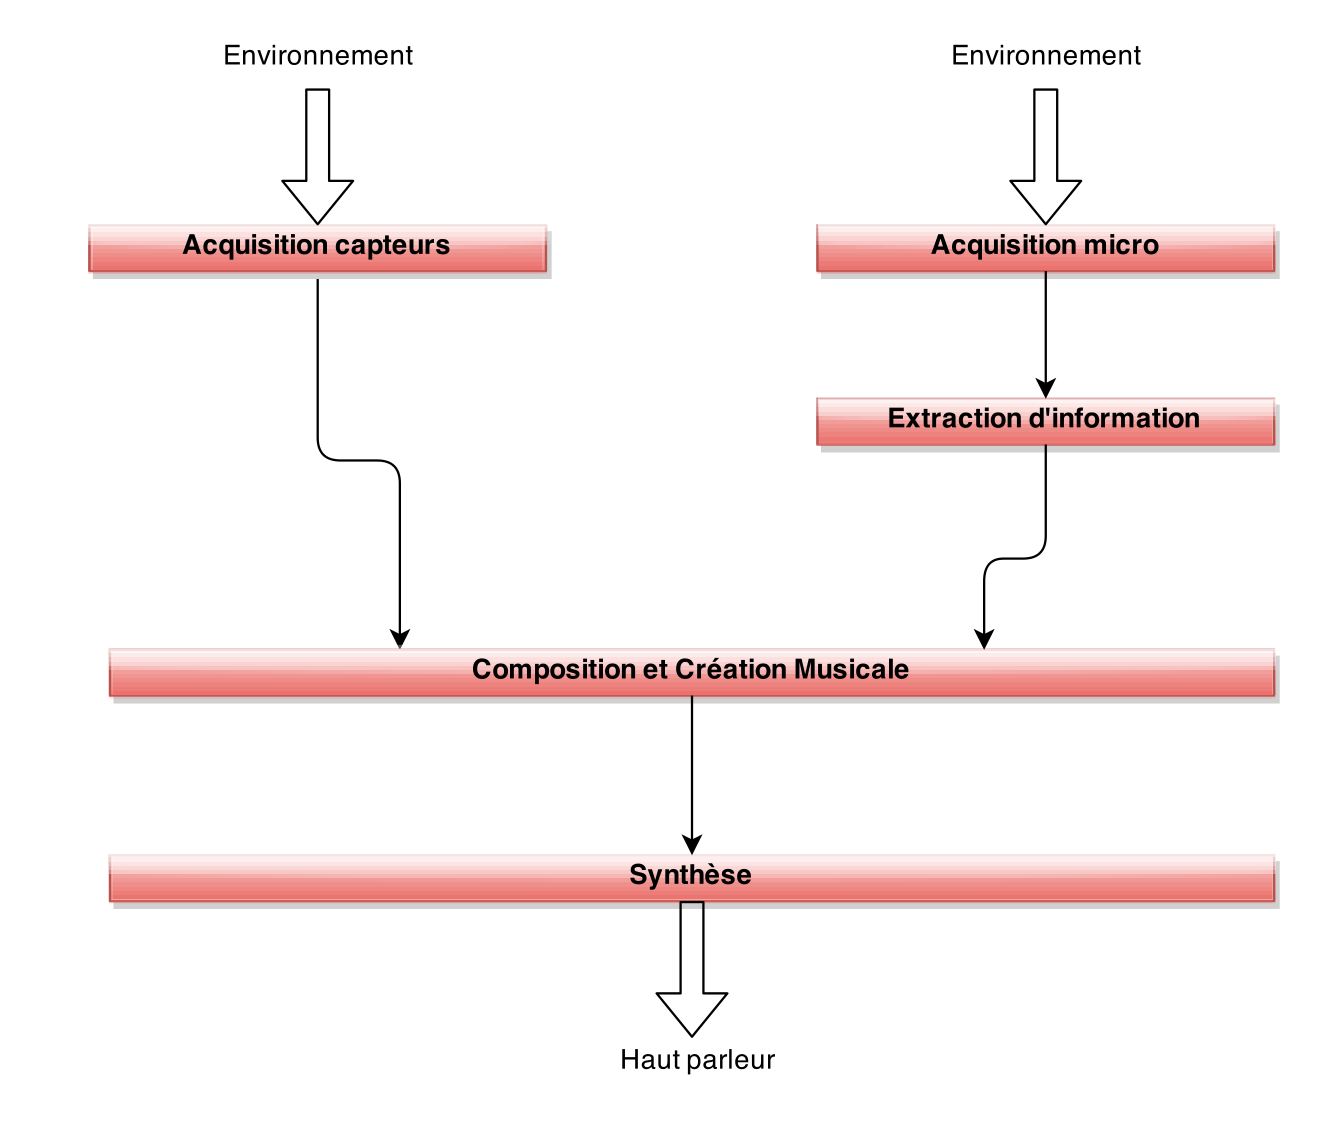
\includegraphics[width=400px]{structprojet.jpg}
\end{figure}

\paragraph{}
La partie acquisition des données des capteurs ce fera par le bien de la communication entre la partie Arduino et Pure Data.\\
Nous avons ecrit un programme arduino qui va envoyé périodiquement les valeurs des différant capteurs au programme Pd.

Information collecté par la partie arduino:
\begin{itemize}
\item Luminosite
\item Temperature
\item Humidité
\end{itemize}

\paragraph{}
Une seconde partie acquisition est la réception du signal sonore, que l'on doit traiter pour pouvoir en extraire des informations pertinente.\\
Le son capté par le micro est pollué par des sons ambiant, typiquement le bruit d'une route proche ou d'une marchine bruyante. Ces bruits sont généralement continu, grave (moins  de 100 hertz) donc très énergétique. Ils peuvent donc fausser les résultats des traitement en aval.\\
 Les buits naturel à cette fréquence sont tres rare dans la nature. De plus musicalement ces bruits sont asses pauvres.\\
Pour toute ces raisons il est préférable de les filtrer. Pour les même raisons, nous avons ajouter un filtrer pour eliminer les fréquences au dessus de 6000 Hertz.


\paragraph{}
Dans la partie extraction, avec le compositeur et le chercheur nous nous sommes questionner sur les informations pertinente a extraire pour la composition musicale.\\ 
En prenant en compte le fait que la carte a un capacité de calcul limité, cela ne permet pas d'avoir de faire tous les traitements complexes.


\paragraph{}
La composition musicale est plus la partie propre au compositeur, et correspond a la partie creation artistique. Plus qu'une fabrication de ce module, la question a etait comment pouvoir permaitre au compositeur de la creer et de pouvoir la modifier sur le dispositif a distance sans ecran ni clavier.

\paragraph{}
Il y plusieurs techniques de synthèse musicale certaine sont plus complexe et gourmand en ressources.\\ Nous avons choisis un synthèse simples car la synthèse etant tres lié a la partie création musicale. Dans ce projet le module de creation musical etant rudimenaire, il en est donc disproportioner de faire un module de synthese tres complexe. 

\paragraph{}
En plus de cette stucture implente dans le dispositif, une interface graphique a etait crée, elle comunique a distante avec le dispositif. L'utilisateur peux envoyer des données pour remplacer les informations recu des capteurs, il peut de egalmenet changer la partie creation musicale.

\section{Récupération de l'environnement}
\paragraph{}
L'un des avantages de la carte Udoo est d'etre compatible Arduino est de proposer les même connectique qu'une Arduino Mega. Cela permet d'utiliser le même langage, d'utiliser les bibliotheques deja écrites ainsi que les mêmes capteurs.\\
De plus la partie  micro controleur etant connecté directement a la partie nano ordinateur via un bus special, la vite de comunication est plus rapide et avec une plus courte latence par rapport a une connexion usb classique.

\paragraph{}
Dans les valeurs envoyés par un capteur deux choses sont interessante, la premiere la valeur et la variation de celci (si elle augmente ou si elle diminue).
\subsection{Dispositif et capteurs}
\paragraph{}
Dans le cadre du projet, seul trois capteurs étaient prevu mais le programme devrait permettre un ajout de capteurs  aisé.\\
Les capteurs utilisés sont des capteurs les plus basique : un capteur de luminosité, de temperature et d'humidité.\\
% photo du montage 
Pour capteur la luminosité, nous avons utilisé une photo-resistance, son fonctionnement est asses simple, plus la luminosité va etre forte plus la resitance interne de composant va etre faible. Il suffit de recupere la tension au borne de composant pour connaitre l'indice de luminosité.\\ 
Malheureusement cette indice ne permet pas de connaitre l'intancité lumineuse en Candela ou en Lux mais permet d'avoir une echelle d'avoir des valeur relavite. Ce qui est suffisant dans le cadre de ce projet.
\paragraph{}
Pour la Temperature et l'humidité le fonctionnement est tres similaire. Contrairement a la luminosité grace a une formule (dépendent de chaque capteur) il sera possible d'avoir la température ou l'hygrométrie précise. 

\subsection{Communication inter plate-forme}
\paragraph{}
Pour la partie micro-controleur l'envoi de donnnées est asses intruitive car il suffit d'ecrire sur le port Série (Serial port), avec des primite d'ecriture basique.\\
Pour la partie ordinateur avec le logiciel Pure Data, il faut utiliser une boite pour se connecter a un périphérique puis on peut lire et ecrire sur celui.\\
La connexion entre l'arduino et Pure data devant etre unique, il a fallu trouver un moyen de pouvoir differensier les données des différant capteur. 
% photo montage du composant

\paragraph{}
Pour communiquer entre les deux parties, j'ai donc define un micro-protocole qui étiquette les données envoyés.\\
Tous les X secondes le programme arduino li les valeurs des capteurs et envoi un message de la forme :
\begin{lstlisting}
NOM_CAPTEURvl: VALEUR;		//vl pour la valeur
MON_CAPTEURvr: VALEUR;		//vr pour la variation
\end{lstlisting}

Pour ajouter un capteur, il suffit d'écrire sur le port série avec un nom de capteur pas encore utiliser et c'est dans la partie Pure data que nous traiterons la nouvelle étiquette.

\paragraph{}
Puis pour il nous ai venu l'idée de permettre à Pure data de pouvoir changer le délai entre chaque envoi de valeur. 
Pour cela il a fallu permettre a l'arduino de pouvoir recevoir des données avec des messages ayant la même forme que l'envoi de donnée avec l'étiquette \texttt{delay}.\\
C'est a ce moment la que nous avons découvert un vice de Pure Data, étant un langage tres faiblement typé. Les donnée recu de l'arduino sont des octets que Pure Data caste en type Nombre et il n'existe pas d'objet permettant a partir de ce flux d'octets de recuperer des integers (valeur des capteurs envoyé par la parite Arduino).\\

Au premiere abord nous avons voulu utiliser l'objet \texttt{PakcOSC} qui permet a la base de convertir un message quelconque en commande OSC (\texttt{Open Sound Control}). Ce protocole etant un protocole avec un codage ascii nous pouvions l'utiliser pour encoder et decoder les communications avec l'arduino. \\
Mais cela aurai ete une manipulation de l'objet de base de plus cela pourrai porter a confusion car nous ne gerions en rien le protocole.\\
Nous avons discuté avec Hugues GENEVOIS et nous avons utilisé de programmer nos prope externals.

\subsection{External pour la communication}
\paragraph{}
En s'inspirant du fonctionnement des objets \texttt{PackOSC} et \texttt{UnPackOSC}, nous avons programmé deux externals, un qui recoi un message et qui le transforme en tableau d'octects (en code ascii plus particulierement) en ajoutant le code ascii d'un point virgule a la fin.\\
Le second recoi un flux d'octets et le stock dans un tableau jusqu'a recevoir un point virgule, a ce momment là il envoi toute la chaine récu.\\
Le fait d'utiliser le caractere ';' n'est pas un probleme car en PureData ce caratere est generalement le delimiter de fin de chaine, la fin de liste et de tableau ainsi quand interne pour fin des messages tcp ainsi que la fin d'une lecture de fichier.

\section{Traitement audio}
\subsection{Aquisition audio}
\paragraph{}
Comme nous l'avons dit dans l'introduction du projet, Nous avons filtré le signal audio capté par le micro pour supprimer les bases frequence et les haut fréquence.\\
Nous avons chercher a savoir determiner les frequences de coupure a partir du quelle il n'y as plus d'information pertinente. Nous nous somme rendu compte qu'au dessus de 6000 Hertz il n'y avait plus de son avec une fondamentale a cette haute, et qu'il n'y avait que des harmonique de son plus grave. (Voir l'annexe rappel musical pour les explications sur les fondamentales et les harmoniques).\\
Pour les sons tres graves, il n'existe pa de sons produits par la nature à des fréquence inférieur à 100 Hertz. Nous avons donc ajouter un filtre a notre acquisition pour pouvoir supprimer les bruits qui pour nous sont des bruits parasites.

\subsection{Traitement du son bas niveau}
\subsubsection{Filtrage}
\paragraph{}
Une inforation qui nous paraissé esentiel a extraire etait les notes et les melodies qui sont jouer dans l'environement.\\
Il est asses facile de determiner la frequence principal d'un signal, il suffit de prendre la forme generale du signal. Il existe plusieurs boites en Pd pour le faire tel que \texttt{Fiddle} ou \texttt{Signum}.\\
Pour detecter les notes jouer simultanement ou suivre plusieurs de melodies simultanement est tres quasiment impossible et fait encore partie l'objet de recherche.\\
L'une des meilleurs compromis entre le temps de calcul et la fiabilité de la sortie est de faire 
En Pd il existe des boites pour déterminer la frequence pour cela nous avons pensé a utiliser la transformé de fourrier (voir Annexe) pour déterminer l'ensemble des notes jouer. \\
Nous avons implémenter un programme en \texttt{C} pour pour faire une transformée Fourrier rapide (FFT), dans l'optique d'en faire une boite pour l'utiliser dans Pure Data mais nous nous sommes rendu compte que ce proceder etait beaucoup trop gourmand pour la carte. Meme si la complexité de la FFT est en Nlog(N), avec N le taux d'echantillonnage du signal (nombre de point du signal). Notre signal est echantilloné a 44k Hertz il y a donc 44100 points a traiter par seconde ce qui est trop lourd pour la carte (si nous voulons pouvoir faire d'autres traitements en parallèle).

\paragraph{}
%TODO faire un graphique 

Apres ces tests insatisfesant, nous nous sommes donc orienter dans une autre direction, le chercheur nous a conseiller de partager le spectre sonore en plusieurs bandes de fréquences a l'aide de filtre passe-band et de suivre de deterter la frequence la plus principal de chaque bande, avec un \texttt{fiddle}.\\
Apres avoir implémenté en pure data ce mecanisme un nouveau probleme est apparu. Les filtres ne coupant pas parfaitement les frequences en dehors de sa bande, les objet \texttt{fiddle} detecter parfois des frequences n'appartennent pas a leurs bande de frequence. Il y avait donc plusieurs filtre qui detecter donc la même frequence ce qui etait asses problematique.\\

\paragraph{}
Pour resoudre ce second probleme nous avons utilisé des noiseGate.\\
Une noiseGate est un element souvant utliser en musique, il correspond simplement a un boite qui ne laisse passer que les signals sonore d'une certaine intensité, si le signal est trop faible le signal en sortie de la boite est egale a 0.
Cela permet de supprimer les sons venant des autres bandes de frequences, etant atenuer par les filtres, ces sons ne passe pas la NoiseGates, ce qui resolvé le problemee de la detection de fréquence erroné.

\subsubsection{Détecteur de notes}
\paragraph{}
Ce dispositif était bien mieux que les précèdent mais ne permettait pas de suivre les melodies qui etait etaler sur plusieurs bandes de fréquences. Ce qui se traduisé par la detection de morceau de melodie souvant haché.\\
Nous avons donc decider d'abandonner l'idée de suivre plusieurs melodie simulanement et de ne garde que la melodie principal du signal. \\
Et de ne n'utilsier les notes récupérer par les filtres uniquement  pour savoir quelle note sont jouer pendant un labse de temps.\\
Ce choix choix peut semblé un peu etonnant mais il est tres important pour le dispositif de savoir quel note son jouer, si la melodie qu'il capte utiliser uniquement deux notes, il serait tres disonnant que le disposirif en joue une troisieme note qui n'a rien a voir avec les deux premieres.\\
Donc implementé un compteur de notes qui collecte les notes reconnues a la sortie des filtres. A intervalle régulier le compteur va nous donner la fréquence des notes joué. Pour ne pas faire trop de dissonnance il suffira au module de synthese de jouer des note tiré au hasard dans la liste de note en tenant compte de la frequence d'apparition d'une note.

\subsubsection{Bandes de fréquences}
\paragraph{}
Avec ce systeme de detection de note, ils est possible de savoir la fréquence d'appartion des notes mais il n'est pas possible de savoir la hauteur des sons capté.\\
Nous avons donc ajouter un module pour mesurer l'amplitude du signal sur chaque bande de fréquence pour savoir où sont reparti les notes sur les bandes de fréquences, si les bruits capté par le micro sont plutot aigue ou grave.

\subsection{Traitement du son haut niveau - Extraction des méta-données}
\subsubsection{Mélodie et rythme}
\paragraph{}
Comme expliqué dans la section percedente, nous avons implementé un module pour detecter la melodie principal du signal.\\
%TODO image pour detection de note
Nous avons donc voulu implementé un module homologue a la detection de note, mais pour déterminer les rythmes. Pour synthetiser du son avec des rythmes proche de l'environement.\\
Concretement si une personne marche pres de du dispositif il peut repondre en jouer des son sur le même rythme ou dans le cas ou le il capte un chant d'oiseau, il peut reponse en jouant des notes semblable avec le même rythme.\\

\paragraph{}
Apres en avoir discuté avec notre encadrant, il nous est apparu que pour connaitre pouvoir detecter un debut de note, la maniere de proceder est de detecter les impacts, generalement caracteristique d'une debut de note. Pour cela  nous avons calcule l'energie du signal (voir annexe). 
% TODO SCHEMA avec seuil max et min
Il suffit ensuite de regarder son evolution, si une augmentation brusque apparait, cela induit la presense d'un impact et donc du debut de note.\\
Pour raffiner la détection d'impact, nous avons ajouter un seuil minimal et manimal a depasser pour considerer que l'evenement est bien un debut de note.
 

\paragraph{}
Dans l'environement les bruit sont intermiant, il nous nous sommes dit qu'il serait interessant de grouper les evenements ryhtmique en sequence. Un sequence commence quand le dispositif detecte le debut d''un note et termine apres un labse de temps sans imparte (de quelque secondes). Pour eviter de faire des sequences trop longeux dans le cas d'un environnement tres bruillant nous avons decider arbitrairement de limiter un mnombre d'evenement maximum dans une sequence (de l'ordre de la centaine).

\paragraph{}
Pour permaitre au dispositif de jouer la même structure rythmique mais a differante vitesse. Nous avons decider de normaliser notre notation de rythme.
%TODO ajoute schema interval  example
Le premier intervalle entre deux notes sera la reference pour toute la sequence, elle aura une valeur "1", tous les autres intervalle seront des multiples de cette valeurs.\\
Avec ce systemes il est possible de mesurer des divisions de cette valeurs jusqu'a la quadruple croche (1/16) ce qui nous parrait etre une precision suffisante.\\
Nous avons rajouter une certaine tolérante au calcule de valeur pour permaitre une certaine approximation dans les rythmes. Il est quasiment impossible de jouer rigoureusement plusieurs notes parfaitement égales.\\
Les sequences dete ter son au final de la forme:\\
\begin{figure}[H]
	\includegraphics[width=100px] {sequence_ryhtmique.jpg}
	\caption{\label{étiquette} Sequence Rythmique detecté}
	\includegraphics[width=140px]{sequence_rytmique_possible.jpg}
	\caption{\label{étiquette} Deux ryhtmes pouvant produire la sequence}
\end{figure}

\subsubsection{Détection de Motif minimal}
\paragraph{}
Nous avons beaucoup discuter de la detection melodie et rythmique avec Hugues GENEVOIS, et nous en avons tirer la conclusion qui serai interessant d'extraire des sequences rythmes les rythme les motifs melodie et rythmique qui revienne dans ce sequence.\\
Cette operation s'averant tres complexe en Pure Data a cause du fait qu'il est compliquer de stocker des données. Nous avons donc decider de faire deux externals un pour les motifs melodie et un pour le motif rythmique.\\
Nous allons vous decrire le fonctionnement detailler de l'external de detection de motif rythmique, il sauf savoir que le l'external pour de detection de motif melodie fonctionne de maniere homologue.\\
On donner en parametre a l'external le nombre minimal du motif. Et nous lui envoyons la sequence rythmique à la volé, des que le module de tection rythmique détecte un nouveau intervalle il est directement envoyer au module de detection de motif rythmqiue.\\
Il stock les valeurs est a chaque recpetion de nouvelle valeur va tester si il n'a pas deja rencontre un motif contenant ce rythme. Des qu'un motif sera detecter l'external va envoyer ce motif rythmique pour qu'il soit utiliser pour la synthese.\\
Ce module ne permet pas de faire reconnaitre la plus long des motifs rythmiques present dans la sequence mais pour pouvoir interagir rapidement avec son environnement, il est preferable d'avoir un motif court, le plus vite possible plutot qu'un motif plus grand mais qu'il faille que la sequence soit terminer et donc que l'interation avec le dispostif soit moindre. Le dispositif n'ayant la plus longue sequence uniquement une fois que l'emetteur a fini de jouer.
% TODO schema detection de motif

\section{Synthèse musical}
\subsection{Modele physique au longterme}
\paragraph{}
La synthèse par modélisation physique consiste à produire des sons à partir d'un modèle informatique décrivant les propriétés physiques d'objets virtuels.\\
On donne les caractéristiqaues physique (dimension, densité, élasticité...) de l'objet que l'on veut simuler, et les caracteristique de objet qui sera l'exitateur. Puis on nous utilison cette  simulation d'instrument pour produire du son. Cela permet d'avoir une timbre de sons tres varier.\\
L'utilisateur de cette synthese a ete evoquer mais ca complexité plus elevé et le temps etant limité nous nous avons preferer faire utliser un modele plus basique.

\subsection{Synthèse implémenté}
\paragraph{}
Pour ce projet, nous avons proceder a un implementation d'un synthese hybride utilusant la synthese additive et soustractive pour generer du son.\
\paragraph{}
La synthese additive consiste a produire un signal audio complexe en additionnent plusieurs signaux elementres (typiquement des ondes sinusoidal).
\paragraph{}
La synthese soustractive quand a elle consiste a produire un signal audio a partir de signaux riche ne harmoniques (comme le signal carré, triangle ou en dent de scie) en filtrant certaine de frequence. 


\section{Interface Utilisateur}
\subsection{Premiere idée d'implementation}
\paragraph{}
Le parametrage du dispositif se faisant a distance, les données sont envoyer au dispositif par wifi la carte udoo etant equipé un module wifi.\\
Comme l'interface graphie et le dispositif communiquaient pas le wifi, nous sommes dit qu'il etait interessant de permettre a l'utilisateur de s'abstraire de la contrainte d'avoir Pure Data sur l'ordinateur configurant le dispositif. \\
Dans l'optique d'avoir une interface portable et simple d'installation, nous avions pensé au Java.
\paragraph{}
En PureData, les communication se sont a l'aide d'une boite du nom de \texttt{netsend} qui permet d'envoyer des messages (Pd) commecent par \texttt{send} et envoie les données a la fin du message. En Tcp ou en Udp selon les parametres de la boites.\\
\texttt{netreceiver}, la boite complementaire de \texttt{netsend}, stock les données recus jusqu'a recevoir la fin du message, et l'envoie sur la sortie de la boite.\\
Dans un premier temps il nous a donc fallu trouver comment Pure Data convertiser les messages avant de les envoyer si il sagié d'une ismple convertion en ASCII ou un autre  mecanisme. De plus il a fallu trouvé le caractere ajouter au message par netsebnd ou que netreceiver puisse connaitre la fin du message.\\
Apres plusieurs experimentations ous avons decouvert que le caratere etait le ';', ce qui nous a permis de faire d'envoyer des messages exterieur (d'une programm) à PureData.

\paragraph{}
Apres quelque teste nous sommes dit que le parametrage du dispositif ne pouvait pas ce faire sans connaissances en Pure Data. Par consequent, nous decider de change d'idéee et de fournir un interface graphique fait en Pure Data, l'utilisateur serai plus a l'aise avec une interface fait dans un langage qu'il connait et qui a la philosophie que le programme embarqué dans le dispositif. L'utilisateur pourra egalement l'adaper selon ses besoins.
%TODO photo de l'affichage graphique
\subsection{Envoie des données capteur}
\paragraph{}
Nous avons recontré plusieurs fois le compositieur pour savoir ce qui lui serait le plus facile pour l'envoie de données. Il lui a paru interessant de dessiner des coubes pour chaque capteur. Il a pense egalement que pouvoir choisir changer la précision des courbes pour pouvoir similer de grande variations ou au contraire des tres petit variation.\\
\paragraph{fonctionnement}
L'utilisateur peut dessinerl les courbes qui desir pour capteur, quand il a fini il se connecte au dispositif a ce moment l'interface envoie les doonées au dispositif qui va les socker et tant que la connectio n'est rompu par l'utilisateur va les lire en boucle et s'en servir comme si ses informations etait celle des capteurs.\\
Pour envoyer de nouvelle données, il suffira a l'utilisateur de tracer de nouvelle courbe, de se deconnecter et de se reconnecte pour que l'envoie de face a nouveau.

\subsection{Envoie d'objet Pure data}
\paragraph{}
En Pure Data, il est impossible de pouvoir modifier un patch autrement que par l'interface du logiciel en ajoutant des boites ou des connections. Et donc la creation du module "Creation Musicale" génerique que l'utilisateur pourrai modelé a ca guise serait impossible a programmer. La Creation d'une mouveau module serait obligatoire pour chaque evenement.
\paragraph{}
Nous nous sommes questionné sur comment  pouvoir changer la partie "Creation musicale" à distance.\\
La premiere chose envisage a etait de faire un simple script \texttt{Bash} pour envoyer un pathc programmé par sur l'ordinateur de l'utilisateur vers le dispositif. Le defaut majeur de cette technique est le cela force l'utilisateur a connaitre les commandes utile pour maintenir le script et les bases du ssh. Ce qui peut paraitre evident pour une personne travaillant dans le domaine de l'informatique mais qui est rare pour les utilisateurs de PureData. Utilisant un langague graphique pour s'abstraire du code informatique. De plus cela  oblige à utiliser un autre outils que Pd.

\paragraph{}
Nous avons vite laisser le problème de coté, par manque de solutions satisfaisante.\\
En effectuant des teste sur l'evoi de données pour les capteurs l'idée mes venu de ne pas envoyer une liste de données (venant des courbes) mais d'envoyer une liste qui serai le contenu d'un fichier, et plus particulierement d'une fichier Pd.\\
L'idée est que l'utiliateur ecrive un module de creation qu'il envoi le ficher par l'interface graphique et que de l'autre cote, le dispositif le recpetion et ecrive est remplace le module de "Creation Sonore" par le fichier recu.
\paragraph{}
Comme le caractere de ceparation dans les fichiers Pd est le point virgule, et que ce point virgule est aussi utiliser en interne pour delimiter les messages, les fin d'envoi... Cela a lecture et le traitement de ce genre de fichier n'a etait sans difficultés.
\paragraph{}
De plus quand nous avons commencer a implementer cette methode nous ne savions pas cela aller vraiment marcher.\\
A notre grande supprime il est tous a fait possible de reecrire des fichiers sans fait planté le patch actuelle chargé. L'inconveniant est que Pure Data ne recharge le contenu de la boite qu'apres fermeture et reouverture du patch le contenant. Il aurai etait possible d'ecrire un external qui par une commande \texttt{Bash} recharger le patch, dans la version action du projet, on est obligé de d'eteindre et de relancer le dispositif.
\paragraph{}
Un second probleme a etait trouvé si le patch envoyé n'est pas un fichier Pure Data ou que la syntagre du fichier n'est pas rigoureusement suivi. Quant Pure Data ce reouvre avec la nouvelle boite cela produit etrangment pas de message erreur, le chargement du patch s'arret et aucun connexion entre le boite ne sont faite. A ce moment, la seul solution est de re-installer toute la partie Pure Data du dispositif.\\
Il aurai ete intersant de programme un external charger de verifier la syntaxe du fichier envoyé a l'aide de \texttt{regexp} mais faut de temps nous n'avons pas eu le temps de le faire.   

\section{Tutoriel et Documentation}
\subsection{Écriture documentation Pure data}
\paragraph{}
Le projet n'etant qu'une permiere version, il est important de fournir un documentation la plus complete sur le fonctionnement de tous les patchs et les externals fabriquer. Pour facilité la comprehention du programme pas les personnes qui travaillerons sur le projet.
\subsection{Écriture du Tutoriel d'installation}
\paragraph{}
Comme beaucoup d'utilisateur de Pure Data on des connaissances limite en informatique, Nous avons ecrit une documentation qui explique pas a pas ce que l'utilisateur doit faire pour pouvoir reproduire le dispositif.\\
Elle decrit la partie Hardware avec les differant montage des capteurs mais aussi la partie Software pour l'installation de la distribution linux, des packets essantiel pours le faire foncionner correctement, ainsi quela description de l'installation de Pure Data et de Flext a partir des sources.

\paragraph{}
Une image de la carte micro sd sera fourmi pour pouvoir mettre en place le dispositif sur la même carte.\\
De plus un tutoriel est present pour pouvoir permetre a un neofite de faire de nouvelle image, si le dispositif venait a changer.
% sauvegarde de carte et tuto

\section{Pour aller plus loin}
\subsection{Tests en environnement reel}
\paragraph{}
Faire des testes sur le son n'est jamais quelques choses de faciles surtout quand il faut les buits envivorant. ces sons etant souvnat de faible intensiter et de nature tres diverse.
Nous tous de même essayer de faire le plus de teste possible que cela soit de son synthetiser par ordinateur ou des enregistre d'environement. Mais il aurait etait interse de teste les dispositif plus emplement dans des conditoon reeln, que nous n'avons pas eu le temps de faire faute de temps. 

\subsection{Tests énergétiques}
\paragraph{}
La carte Udoo malgrés tous c'est avantage et par toute ca connection et le micro controleur pour un nano-ordinateur. Même si sur certaine document non officiel, estime la consomation moyenne d'energie de la carte a environs 10 Watts. Les specifications et les divers documents officiel trouvé parlent d'une consomation maximum de 24 Watts.\\
Ce qui est considerable pour dispositif devant etre le plus autonome energetique energetiquement.\\
Il aurait etait interessant de faire des testes avec d'autres cartes moins gourmandes en energie.\\
Comme par example combiné une carte Arduino Nano pour l'aquisition de données et un Raspberry Pi V2 pour les traitement, consomerait moins de 5 Watts (environ  0.5 Watts pour l'Arduino et 4 pour la Raspberry).\\
Des testes des programmes sur d'autre platforme et voir si la traitement pourrai se faire en temps reel.

\subsection{Serveur distant}
\paragraph{}
Dans l'optique d'etre de diminuer la consomation d'energie, il aurait peut etre possible d'essayer une implementation centraliser. La carte n'aurai pour role que de collecer les donné pour les envoyer a un serveur qui lui ferrai les traitement et renveré la flux audio ou simplement les parametres a la carte pour synthetiser du son.\\
Cela permaittre de ne plus ce soucier du temps de calcul et permaitre d'avoir une supervision des dispositifs. De plus il serait possible de partagerdes capteurs entre plusieurs dispositifs, comme la pression qui varie que tres peu dans un endroit donné.\\
La modification des modules de creation musical serai egalement simplifié.
 

\newpage
\section{Bibliographie}
\nocite{*}
\bibliographystyle{plain}
\bibliography{biblio-projet-DASS}
%\addcontentsline{toc}{chapter}{Bibliographie}

\newpage\section{Annexe}
\subsection{Rappel musical}
% rappel sur les harmoniques 

\end{document}